\begin{definition}[\cite{barr1990category}]
    \label{def:graph:unlabeled}
    An \textbf{unlabeled graph} \( G \) consists of a collection of \textbf{nodes} (also called \textbf{objects}) and a collection of \textbf{edges}, each equipped with a \textbf{source} (or \textbf{domain}) node and a \textbf{target} (or \textbf{codomain}) node. 
    For an unlabeled graph \( G \), we denote by \( V(G) \) its collection of nodes, \( E(G) \) its collection of edges, \( \operatorname{dom}: E(G) {\to}V(G) \) the domain function, and \( \operatorname{cod}:E(G) {\to} V(G) \) the codomain function. An unlabeled graph is \textbf{finite} if \( V(G) \) and \( E(G) \) are both finite sets. 
    We write \( a: s \to t \) to indicate that \( a \) is a directed edge from \( s \) to \( t \).
\end{definition}   

\begin{example}
    In an unlabeled graph, edges are directed and will be visualized as arrows; between any two nodes, there can be multiple edges, and loops are allowed. An unlabeled graph is depicted in~\autoref{fig:preliminaries:unlabeled_graph} where nodes are marked with numbers to facilitate discussion, but in general, nodes are not labeled.
    \begin{figure}[hbtp]
        \centering
        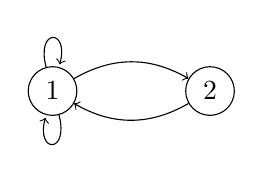
\begin{tikzpicture}
            \graphbox{}{0mm}{0mm}{32mm}{28mm}{-10mm}{-14mm}{
                \node[draw,circle] (1) at (0,0) {1};
                \node[draw,circle] (2) at (2,0) {2};
                \draw[->] (1) edge[loop above] (1) ;
                \draw[->] (1) edge[loop below] (1) ;
                \draw[->] (1) edge[bend left] (2)  ;
                \draw[->] (2) edge[bend left] (1)   ;
            }
        \end{tikzpicture}
    \caption{Unlabeled graph}
    \label{fig:preliminaries:unlabeled_graph}
    \end{figure}
\end{example}